%!TEX options = --shell-escape
\documentclass[notitlepage,10pt]{report}
\usepackage[left=0.75in, right=0.75in, top=0.75in, bottom=0.75in]{geometry}
\usepackage{amssymb}
\usepackage{bondgraphs}
\usepackage{multicol,caption}
\usepackage{titling}
\usepackage{graphicx}
\graphicspath{ {images/} }
\renewcommand{\abstractname}{\vspace{-\baselineskip}}
\newenvironment{Figure}
  {\par\medskip\noindent\minipage{\linewidth}}
  {\endminipage\par\medskip}
\title{Modelling a Crankshaft-Magnetomotive Force System}
\author{Ramandeep Farmaha 20516974\\ Kush Thaker 20517901\\ Siddhanth Unnithan 20523022}
\date{\today}
\begin{document}
\maketitle
\begin{abstract}
\normalsize
The system consists of two subsystems: an inertial wheel with an attached crankshaft arm, and a cart and spring, which are connected by a magnetomotive force created by two magnets. Through constructing a bond graph, the resulting system was then simulated using Python to output the generated force and cart displacement. While the simulation better represented the ideal system than the prototype, it did not account for torque being dependent on the damping and spring coefficients of the torsional spring. Further improvements to the simulation would be to include a nonlinear model of torsion.
\end{abstract}
\begin{multicols}{2}
The designed system consists of two components: an inertial wheel with a crankshaft arm attached, and a cart mass with a spring. Railings are used to constrain the wheel arm, cart and springs in the x direction. A pair of strong magnets are attached to the wheel arm and cart. As torque is applied to the wheel, the crankshaft arm moves towards the cart, and a magnetic force is applied to the second component of the system. The force causes the cart to flow towards the springs and rebound along the rail. The cart may achieve oscillation between the crankshaft arm and springs, but this depends on the strength of the magnets, distance between the cart and springs, and the damping due to friction.
\begin{Figure}
 \centering
   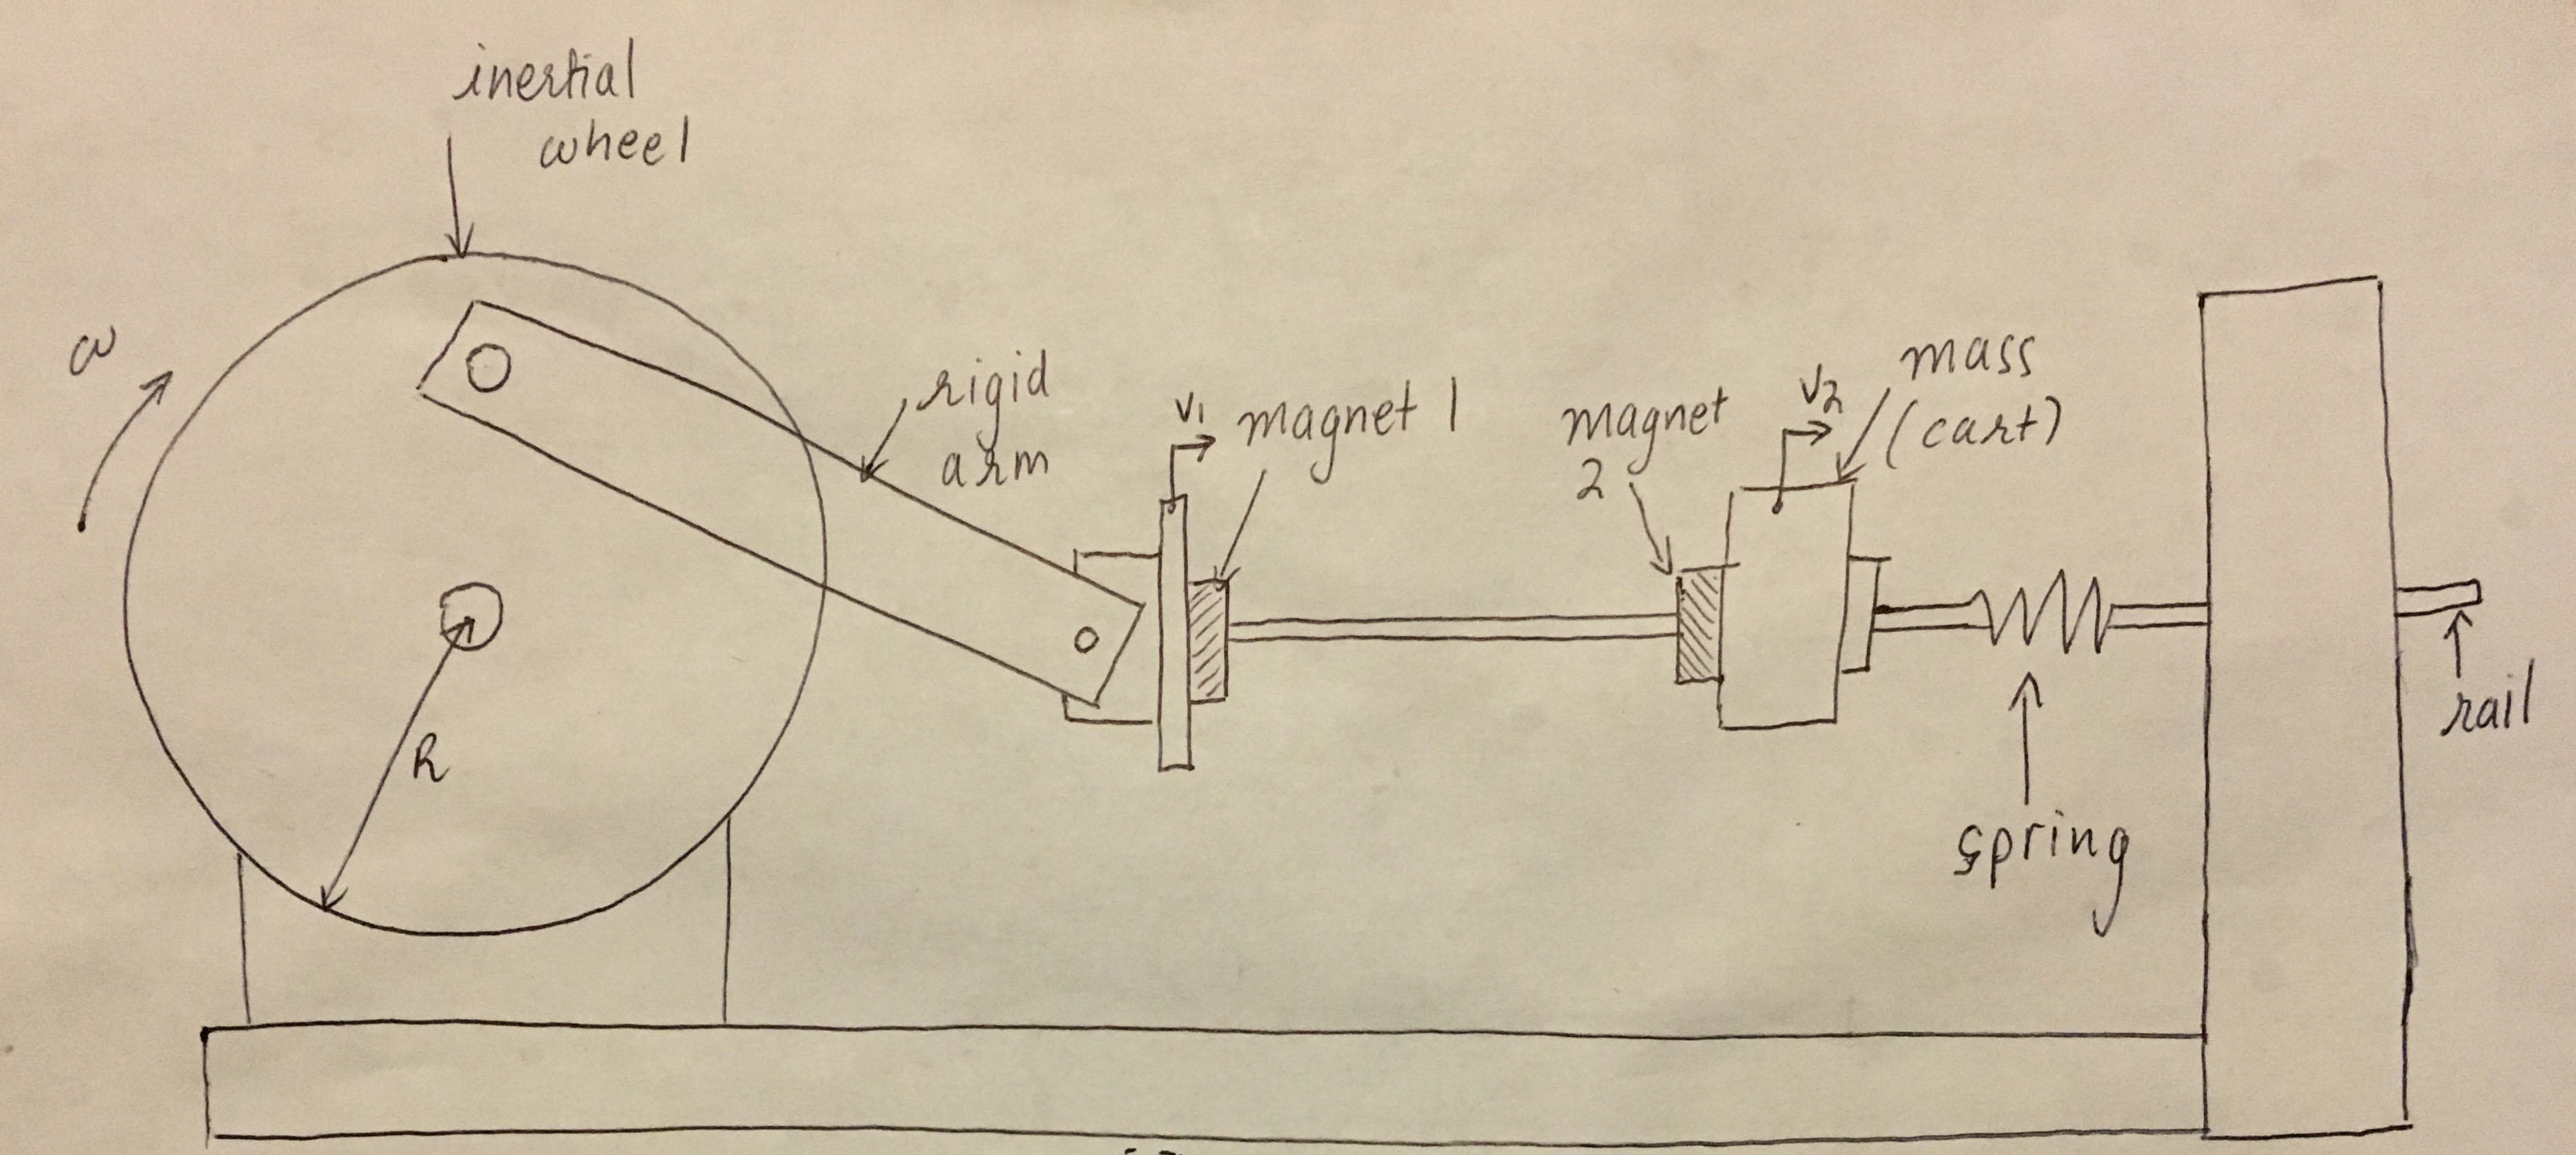
\includegraphics[width=\linewidth]{schematic}
   \captionof{figure}{System Schematic}
   \label{fig:systemSchematic}
\end{Figure}
The prototype was constructed with a large wooden wheel, that can be turned by the system operator. Metal rods were installed as rails to align the direction of the crankshaft arm, cart and springs. The cart was simply a block of wood with screwed in eye bolts. Physically converting rotational motion into linear motion was trickier to implement. The rigid arm length had to be precise to enable the wheel to rotate without interference while being close enough to the cart to push into the springs. Finally, one magnet was glued to the crankshaft arm, while the other was placed on the cart. The physical prototype was adjusted by installing a handle to provide a manual source of flow. The simulated model uses a torsional spring to provide torque instead, thus remaining consistent with the bond graph.
\begin{Figure}
 \centering
   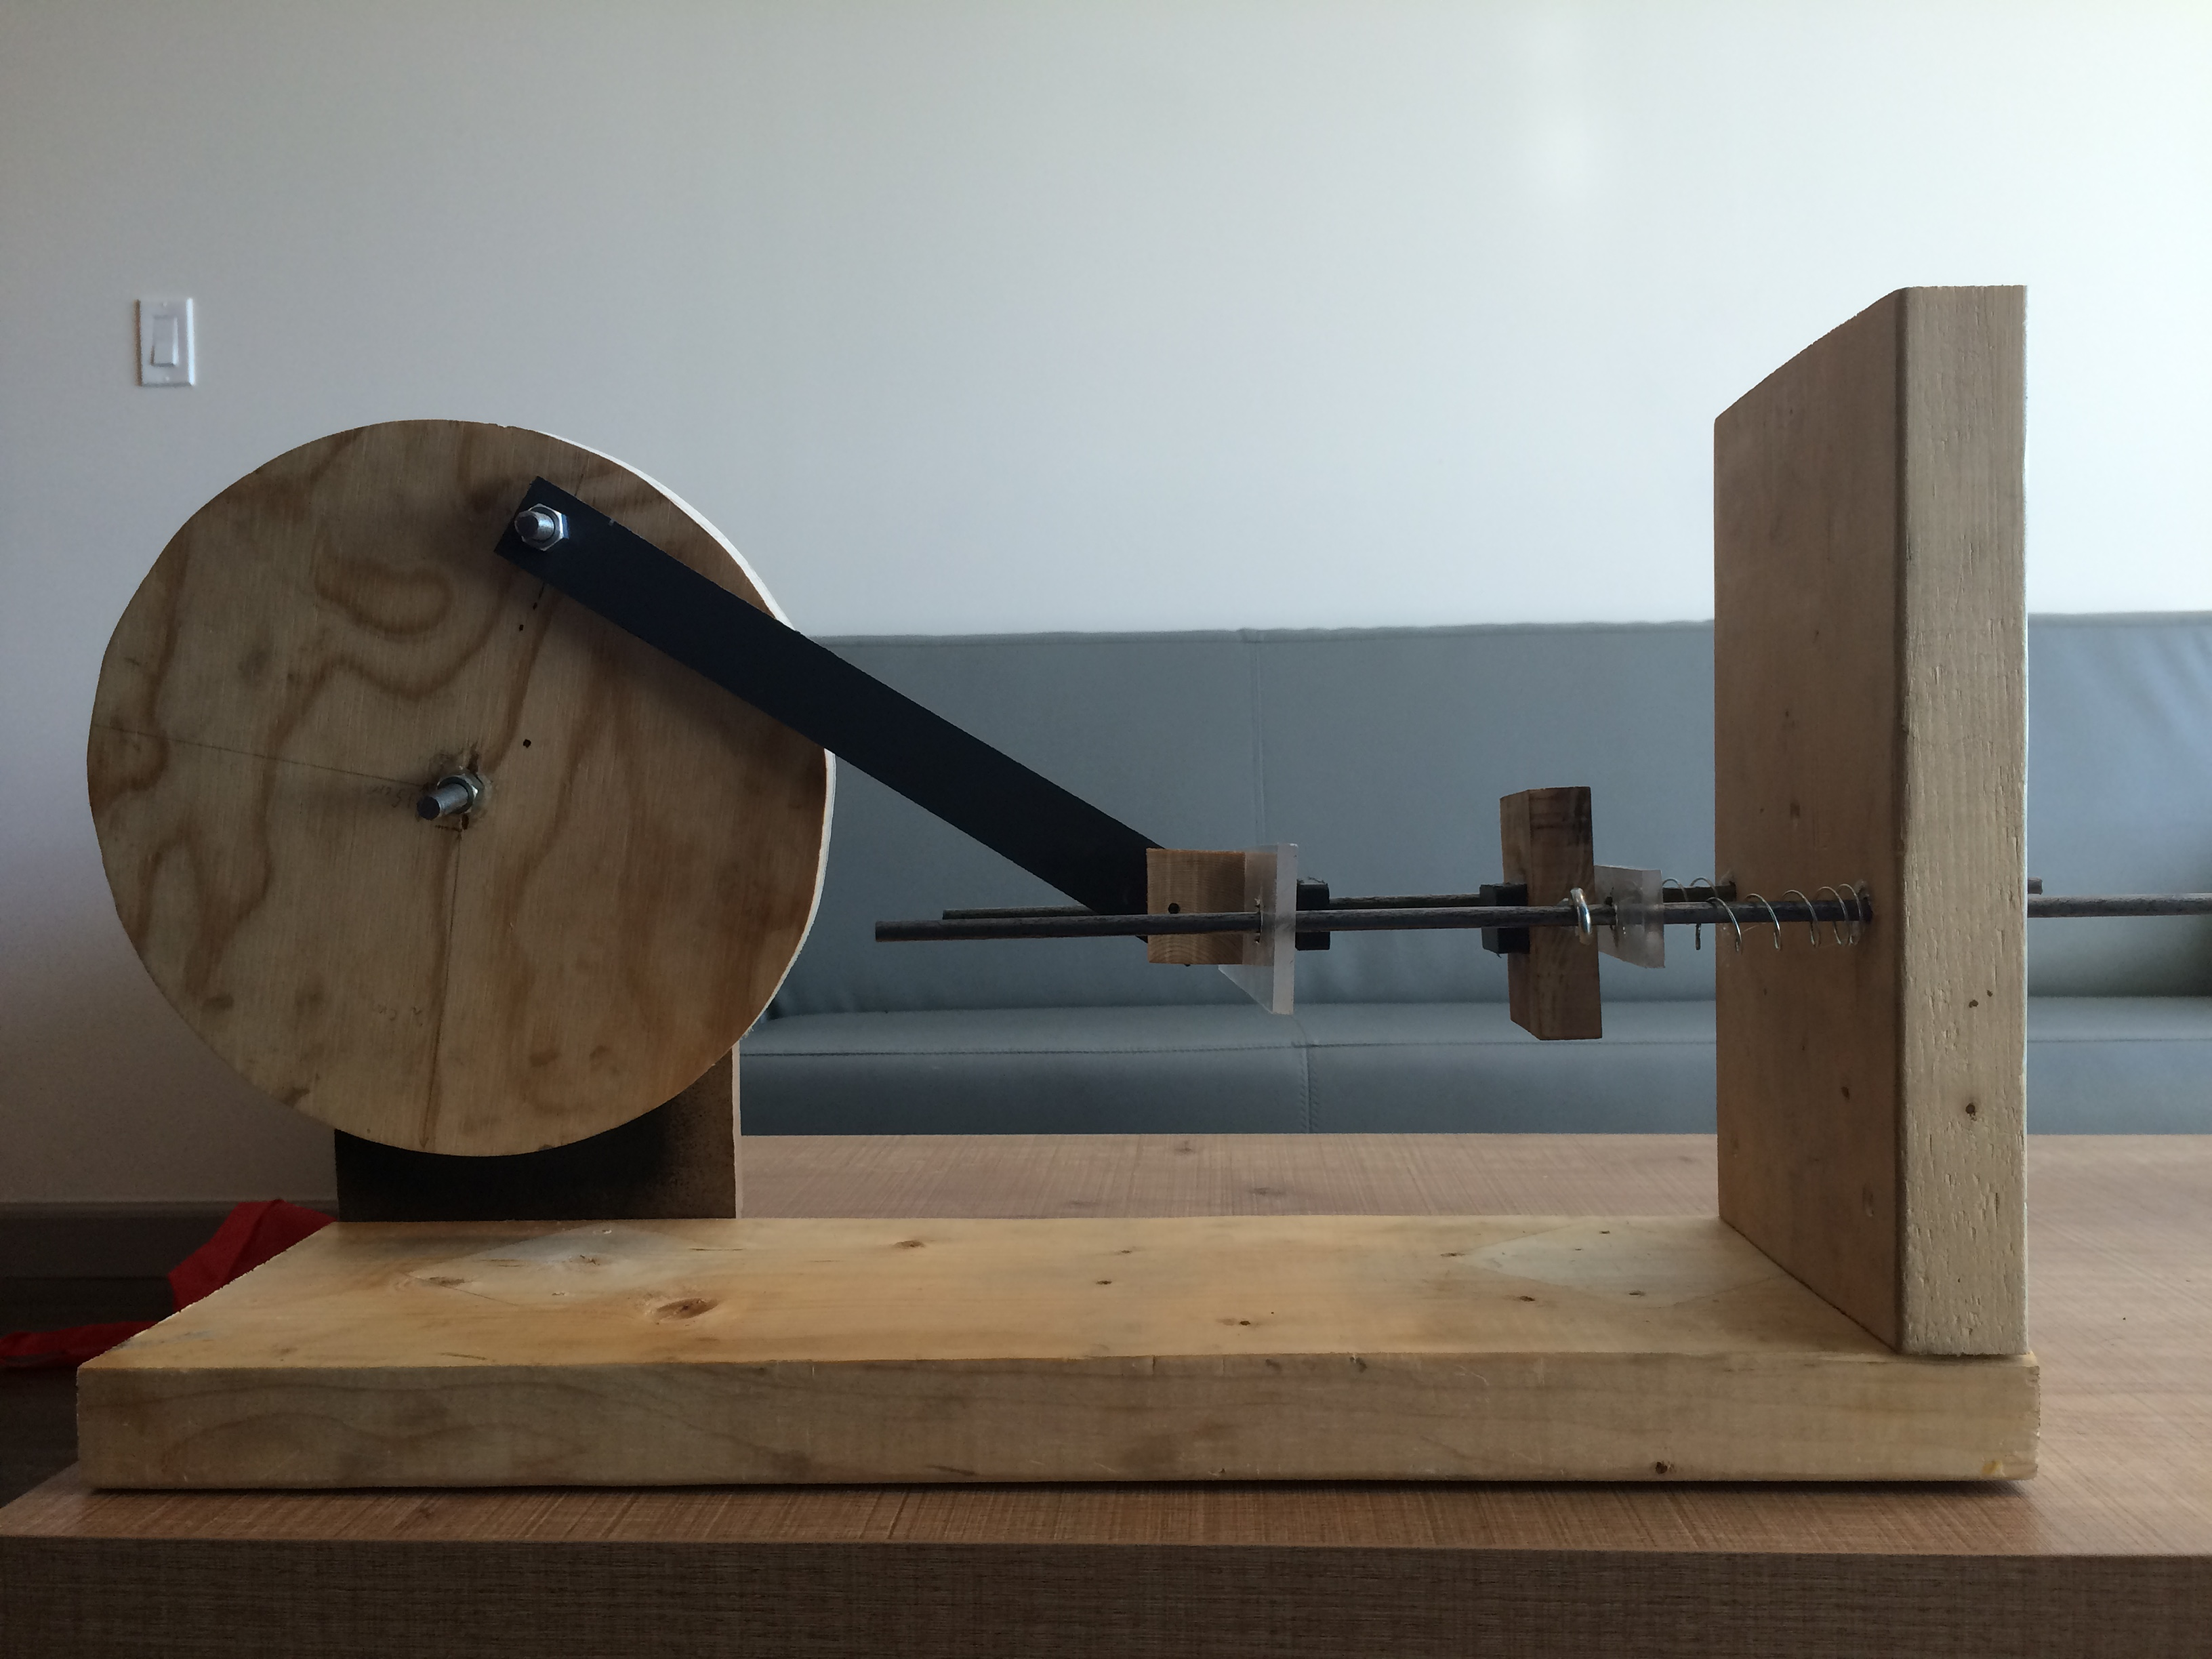
\includegraphics[width=\linewidth]{prototype}
   \captionof{figure}{Constructed Prototype}
   \label{fig:constructedPrototype}
\end{Figure}
There were also problems encountered in applying the theoretical system into practice. For one, the friction was too great along the rails, causing the crankshaft arm and cart to slide unsmoothly. Friction could have been reduced by using ball bearings to slide against the rails. Next, the springs were too stiff, limiting the cart’s rebound motion. A spring with a lesser k value could compress further and exert a greater rebound force on the cart. Thirdly, the strength of the magnets was too small to push the cart into the springs with enough force. Like decreasing the spring’s stiffness, a greater repelling force applied to the cart could also have created a preferred rebound motion. These problems together limited the cart from oscillating along the rail as desired.

The bond graph model consists of two subsystems, the first of which is the inertial wheel. A source of torque is provided to a 1 junction, into the rotational inertia of the wheel, and into a transformer (TF) element. The rotational motion is converted to linear motion here. The TF element flows into another 1 junction, and thus into the inertial element representing the mass of the first magnet. As a source of effort creates mandatory causality at the first 1 junction, the first magnet mass is in derivative causality. 
% Initial bondgraph
\begin{figure*}
   \centering
   \tikzstyle{block}=[minimum width=7mm,minimum height=7mm,draw,thick]
   \tikzstyle{signal} = [-latex, color=red!30!black]
   \begin{tikzpicture}
      \node[bgelement, label=north:$mmf_i$$_n$] (Se) at (0,0) {SE};
      \node[bgelement] (one) at (2,0) {1};
      \node[bgelement, label=right:$\frac{1}{k}$] (C) at (4,0) {C};
      \node[bgelement, above=1 of one, label=north:$m_m$$_2$] (I) {I};
      \node[bgelement] (oneright) at (-3, 0) {1};
      \node[bgelement, above=1 of oneright, label=north:$m_m$$_1$] (Im1) {I};
      \node[bgelement, left=1 of oneright, label=south:R] (TF) {TF};
      \node[bgelement, left=1 of TF] (oneleft) {1};
      \node[bgelement, above=1 of oneleft, label=north:J] (IJ) {I};
      \node[bgelement, left=1 of oneleft, label=south:$T_i$$_n$] (SEin) {SE};
      \node[block,below=1 of TF] (int) {$\int$};
      \node[block,right=1 of int] (ddt) {$\theta$};
      \draw[bond,f_in] (Se) -- node[pos=0.5,above]{$w$} (one);
      \draw[bond, f_in] (one) -- (I);
      \draw[bond, f_out] (one) -- (C);
      \draw[bond, f_out={error}] (oneright) -- (Im1);
      \draw[bond, f_out] (TF) -- (oneright);
      \draw[bond, f_out] (oneleft) -- (TF);
      \draw[bond, f_in] (oneleft) -- (IJ);
      \draw[bond, f_in] (SEin) -- (oneleft);
      \begin{scope}[every path/.style={signal}]
            \draw (oneleft) -- node[pos=0.5,right]{$w$} (int);
            \draw (int) -- (ddt);
            \draw (ddt) -- (Se);
         \end{scope}
    \end{tikzpicture}
    \caption{Bondgraph modelling magnetomotive force as SE}
    \label{fig:bondgraph1}
\end{figure*}
The second subsystem is the cart and spring. The source of effort, or magnetomotive force, of this subsystem is a function of the distance between the magnet on the crankshaft arm and the cart mass, which in turn is a function of the angular displacement of the inertial wheel. This source of effort flows through a 1 junction into an I element, the cart mass, and C element, the spring. The second subsystem contains all integral causalities, as desired. 

The major measured parameters were the radius of the wheel, the masses of the cart, wheel and magnets, and the length of the crankshaft arm. The spring constant was derived to be roughly 89.1 N/m by attaching a one-pound weight to the springs and measuring the vertical displacement. The magnetomotive force was calculated using the following equation: 
\begin{equation}
   F=\bigg[\frac{B_0^2A^2(L^2+R^2)}{\pi\mu_0L^2}\bigg]\bigg[\frac{1}{x^2} + \frac{1}{(x+2L)^2} - \frac{2}{(x+L)^2}\bigg]
\end{equation}

The bar magnets were idealized as cylindrical in order to simplify the calculation, with a radius equal to half their width and the measured length. As noted before, this magnetomotive force is calculated using the separation of the two magnets, which is dependent on the position of the crankshaft and the moving cart.

As the bond graph in Figure ~\ref{fig:bondgraph1} presents two systems of interest, there exists two sets of state variables for modelling. The first system consists of an angular momentum resulting from the inertial mass of the wheel. The second system includes momentum and displacement related to the cart mass and spring, respectively. The final state variable is the measured angle between the crankshaft arm and the symmetric center-line of the wheel. As the magnetomotive repelling force remains a function of the measured angle, the model treats said angle as a state variable. 

The derived state equations for the model are listed below. It should be noted that each of the state equations is in explicit form, thus reflecting resolved derivative causalities.

\begin{equation}
   \frac{dp_2}{dt} = \frac{T_{in}}{1 + \frac{R^2}{J}m_{m_{1}}}
\end{equation}
\begin{equation}
   \frac{dp_9}{dt} = \frac{mmF(x) - \frac{1}{k}q_8}{1 + \frac{m_{m_{2}}}{m}}
\end{equation}
\begin{equation}
   \frac{dq_8}{dt} = \frac{1}{m}p_7
\end{equation}
\begin{equation}
   \frac{d\theta}{dt} = \frac{1}{J}p_2
\end{equation}
The magnetomotive force in Equation 1 was chosen to be one of the outputs of interest, due its relation with the angular displacement of the wheel and the input torque provided to the first subsystem. Velocity of the cart was computed using its momentum and mass, thus enabling the calculation of the second output of interest: cart displacement.  
\begin{Figure}
 \centering
   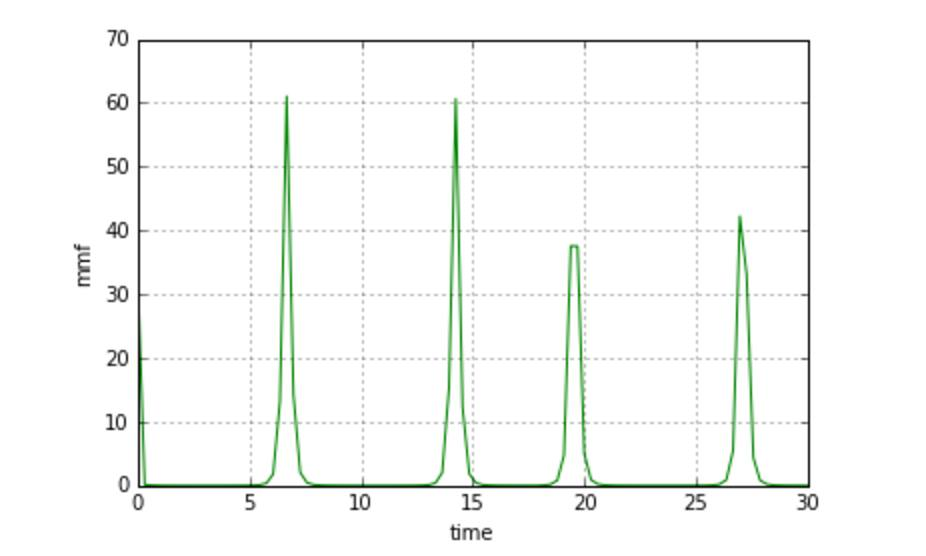
\includegraphics[width=\linewidth]{magnetomotive}
   \captionof{figure}{Magnetomotive Force vs. Time}
   \label{fig:magForce}
\end{Figure}
\begin{figure*}
   \centering
   \tikzstyle{block}=[minimum width=7mm,minimum height=7mm,draw,thick]
   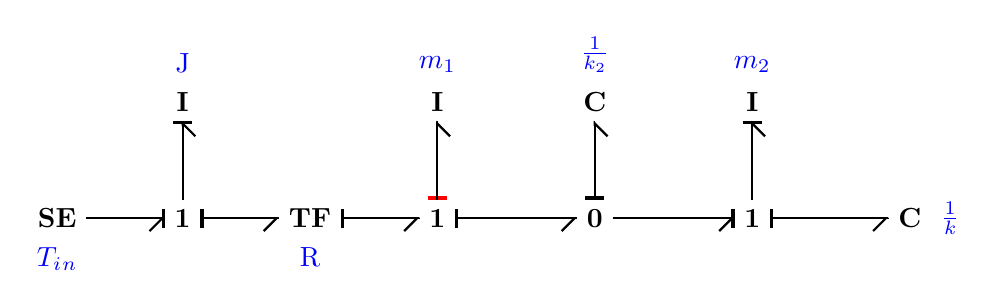
\begin{tikzpicture}
      \node[bgelement] (0bond) at (0,0) {0};
      \node[bgelement] (one) at (2,0) {1};
      \node[bgelement, label=right:$\frac{1}{k}$] (C) at (4,0) {C};
      \node[bgelement, above=1 of one, label=north:$m_2$] (I) {I};
      \node[bgelement] (oneright) at (-2, 0) {1};
      \node[bgelement, above=1 of oneright, label=north:$m_1$] (Im1) {I};
      \node[bgelement, left=1 of oneright, label=south:R] (TF) {TF};
      \node[bgelement, left=1 of TF] (oneleft) {1};
      \node[bgelement, above=1 of oneleft, label=north:J] (IJ) {I};
      \node[bgelement, left=1 of oneleft, label=south:$T_i$$_n$] (SEin) {SE};
      \node[bgelement, above=1 of 0bond, label=north:$\frac{1}{k_2}$] (C2) {C};
      \draw[bond,f_in] (0bond) -- (one);
      \draw[bond, f_in] (one) -- (I);
      \draw[bond, f_out] (one) -- (C);
      \draw[bond, f_out={error}] (oneright) -- (Im1);
      \draw[bond, f_out] (TF) -- (oneright);
      \draw[bond, f_out] (oneleft) -- (TF);
      \draw[bond, f_in] (oneleft) -- (IJ);
      \draw[bond, f_in] (SEin) -- (oneleft);
      \draw[bond, f_out] (oneright) -- (0bond);
      \draw[bond, f_out] (0bond) -- (C2);
    \end{tikzpicture}
    \caption{Revised Bondgraph}
    \label{fig:bondgraph2}
\end{figure*}
Using Python, the behaviour of the system was simulated and plots were drawn to showcase outputs of interest. The following plots display the generated magnetomotive force and resultant cart displacement over a fixed period of time. As observed in Figure ~\ref{fig:magForce}, the peaks of the magnetomotive force correspond to time intervals during which the distance between the first magnet and the cart mass decreases. The impulse-like behaviour of the magnetomotive force is reasoned through the inverse relationship between the force and the squared distance between the two magnets.

In the ideal model, the movement of the inertial wheel and the torsional spring is described by the following differential equation: 
\begin{equation}
   J\frac{d^2\theta}{dt^2} + C\frac{d\theta}{dt} + K\theta = T_osin(\omega t)
\end{equation}
which can be solved for $\theta$ and would provide a nonlinear differential equation that is in terms of K, the spring constant, B, the damping coefficient of the spring, and J, the mass moment of inertia of the wheel. Thus, the torsion of the spring, which is a product of J and $\alpha$, the acceleration of the inertial mass, is nonlinear since $\alpha$ is a function of theta. This nonlinear model is too complex for the context of this report, instead, we idealize the torsion of the spring as linearly decreasing at an arbitrary rate from some maximum torque. 
\begin{Figure}
 \centering
   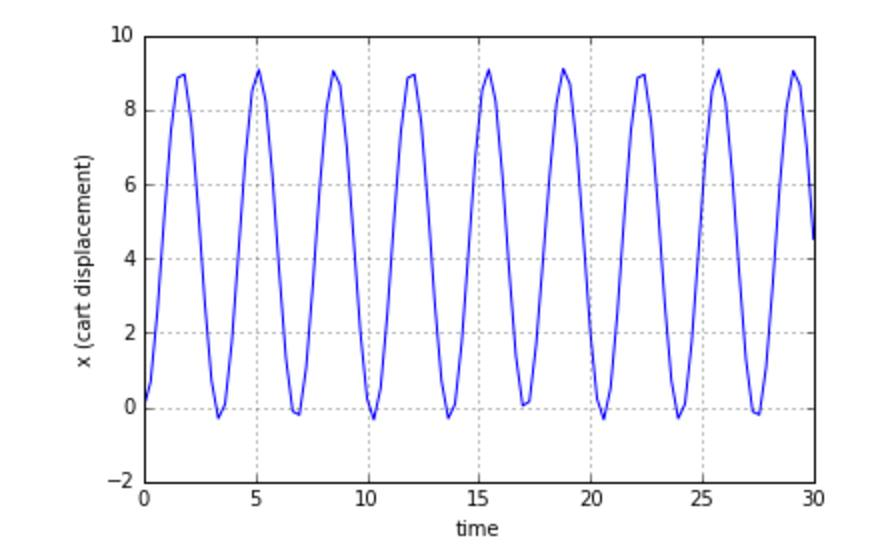
\includegraphics[width=\linewidth]{displacement}
   \captionof{figure}{Cart Displacement vs. Time}
   \label{fig:cartDisplacement}
\end{Figure} 
Since torque is idealized as linearly decreasing, the model doesn’t account for the damping or the effect of the mass moment of inertia on the torsional spring. This is evident in Figure ~\ref{fig:cartDisplacement}, which shows that the displacement of the cart is strictly sinusoidal with no perceivable damping. Ideally, the cart should follow a sinusoidal path with underdamping due to the damping coefficient of the spring.

The prototype, however, demonstrates overdamping, due to the high friction in the rails that the cart sits on, and the high stiffness of the springs. To replicate a system similar to the model, bearings could have been used to reduce the friction between the cart and the rails, which would decrease the amount of overdamping in the system. Also, springs with lower spring constants should have been used, which would also have reduced the amount of damping in the system, possibly allowing for an underdamped system. To retrieve better test data, a photographic tracking software package such as Tracker could have been used, which would have allowed us to plot the movement of the cart in real time. This data could then be verified with the simulation data, rather than relying on human observation.

An alternative to the initial bond graph is one which consists of a capacitance element in place of the MMF, as seen in Figure ~\ref{fig:bondgraph2}. The difference between velocities of the first magnet and the cart-mass is represented through a 0-junction. The stored energy, resulting from the interaction between two repelling magnet poles, can be modelled through a C-element; in the magnetic domain, the C-element is representative of the permeability of free space between the two magnets. A transformer remains applicable in the newly constructed bond graph as the rotation of the inertial wheel is still being transformed into the horizontal velocity of the first magnet. This horizontal velocity then drives the stored energy of the newly added capacitance element, which in turn provides a differential velocity to the cart-mass.

\end{multicols}
\end{document}  